\documentclass[12pt, letterpaper]{article}
\usepackage[utf8]{inputenc}
\usepackage[margin=1in]{geometry}
\usepackage{amsmath}
\usepackage{amssymb}
\usepackage{fancyhdr}
\usepackage{pgfplots}
\usepackage{graphicx}
\usepackage{mathtools}
\usepackage{cancel}
\usepackage{cite}
\pgfplotsset{compat=1.16}
\graphicspath{ {./pictures/} }

\title{Portofolio Assignment 1}
\author{Candidate: 25}
\date{September 2020}

\pagestyle{fancy}
\renewcommand{\headrulewidth}{0pt}
\renewcommand{\footrulewidth}{0pt}

\fancyhf{}
\rhead{
    candidate: 25\\
}
\rfoot{Page \thepage}

\begin{document}
  \maketitle
  \thispagestyle{fancy}
  \section*{Problem 1}
    \subsection*{(1a)} \\
      Supervised learning consists of machine learning algorithms which both has inputs and outputs. The goal of the supervised learning algorithm is using the observed values of $x$ to make an prediction of $y$, where we, the creater of the algorithm is the supervisor. So generally the algorithm consists of whats called a mapping, or the algorithm, of $x$ to $y$. Or we can generalize this as $y = f(x)$, where $f$ is the mapping of $x$ to $y$. Examples of supervised learning algorithms include classification, regression etc. In supervised learning we need to have a training set of labeled data, which means we need to know if a result is correct or not beforehand. We use the labeled data to estimate our parameters.\\
      \newline
      Whereas in unsupervised learning the goal of the algorithm is to find connections in the input data, such that we can learn more from it. Here we don't have a supervisor, we simply try to better see patterns in the input data. We also aren't interested in any output since the input is used to train the model to rule out differences of the variables.\\
      \newline
      We have several ways to evaluate our supervised learning algorithms, the most useful one is the confusion matrix, which works for any number of classes. For two class problems we have even more ways of evaluating the performance of an algorithm. Some are just different names for the same thing, but used in different fields of applications. In general for two class problems though, we can use the confusions matrix to calculate all the other performance measures. We will meet some later in this task, like the confusion matrix, and use it to further calculate the accuracy, precision and recall of our algorithm.\\
      \newline
      The PageRank algorithm is an unsupervised learning algorithm because we do not have labeled training data. We use a probability matrix with only inputs to rank pages in relation to each other. This makes it unsupervised.
      \newline
    \subsection*{(1b)}
      We are given an equation representing the PageRank method,
      \begin{align} \label{eq1}
        r(P_i) = \sum\limits_{P_j \in B_{P_i}} \dfrac{r(P_j)}{|P_j|}.
      \end{align}
      This sum ranks, with the $r(P_i)$ method, the given page, where $p_1, p_2, ... , p_n$ represent all the pages we want to compare against, where $n$ is the number of pages. $P_j$ is a page contained within the set of all the other pages that links to $P_i$, denoted $B_{P_i}$. Then the same is true for $r(P_j)$ as is for $r(P_i)$. $|P_j|$ represents the number of links from $P_j$ to other pages, often called outlinks.\\
      \newline
      This equation will provide a ranking vector, $\pi$, to all the pages $p_1,...,p_n$. That means we need $n$ of these rankings to compute all the ranks for the different pages.\\
      In a sense we can view this as a way for each page to cast a \textit{vote} for the other pages, but it's altered in a way that we can see in equation \ref{eq1}. What happens here is that to give a rank to page $i$, we sum all the ranks of the other pages that link to page $i$, and divide each of those pages rank by their outlinks. If we now say again that each page can cast a vote for another page, then the rank gained by page $i$ from a particular page $j$ is the vote, divided by the other votes page $j$ has casted to other pages.
    \subsection*{(1c)}
      For this problem I'll show an example i think makes everything a bit clearer.\\
      \quad We are given 3 pages: $P_1, P_2, P_3$
      \begin{figure}[h]
        \caption{Illustration of the example}
        \centering
        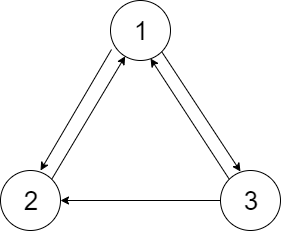
\includegraphics[width=6cm, height=5cm]{Page}
      \end{figure}
      \newline
      This system gives the transitionmatrix, $H^T = $
      \begin{bmatrix}
        0 & 1 & 1/2\\
        1/2 & 0 & 1/2\\
        1/2 & 0 & 0
      \end{bmatrix}
      . \\\newline Where the first column represents $P_1$'s votes for $P_2$ and $P_3$. We note that $P_1$'s votes have been divided by the total number of votes $P_1$ has given. This also goes for the second and third column. This means if we write this as equation (\ref{eq1}) we get the system:\\
      \begin{align} \label{eq2}
        \begin{split}
          r(P_1) & = \dfrac{r(P_1)}{|P_1|} + \dfrac{r(P_2)}{|P_2|} + \dfrac{r(P_3)}{|P_3|}\\
          r(P_2) & = \dfrac{r(P_1)}{|P_1|} + \dfrac{r(P_2)}{|P_2|} + \dfrac{r(P_3)}{|P_3|}\\
          r(P_3) & = \dfrac{r(P_1)}{|P_1|} + \dfrac{r(P_2)}{|P_2|} + \dfrac{r(P_3)}{|P_3|}\\
          &\Downarrow\\
          r(P_1) &= r(P_2) + \dfrac{r(P_3)}{2}\\
          r(P_2) &= \dfrac{r(P_1)}{2} + \dfrac{r(P_3)}{2}\\
          r(P_3) &= \dfrac{r(P_1)}{2}\\
        \end{split}
      \end{align}
      Which look suspiciously similar to a matrix system of equations.
      Let's define a vector $\pi$, such that, \\
      \vskip0.5cm
      $\pi = $\begin{bmatrix}
        r(P_1)\\
        r(P_2)\\
        r(P_3)
      \end{bmatrix}
      , then we see that equation (\ref{eq2}) is the system $H^T \pi$\\
      Which means that $H^T \pi = $
      \begin{bmatrix}
        r(P_2) + \dfrac{r(P_3)}{2} \\ \dfrac{r(P_1)}{2} + \dfrac{r(P_3)}{2} \\ \dfrac{r(P_1)}{2}
      \end{bmatrix}
      $=$
      \begin{bmatrix}
        r(P_1)\\r(P_2)\\r(P_3)
      \end{bmatrix}
      $ = \pi \quad(\Rightarrow \lambda = 1)$\\
      \\
      Which is our eigenvector. Here we see that the transition matrix is just a matrix that holds the votes from a page to another divided by all votes of the page. This example also holds for the general case with $n$ pages.\\
      To solve this as an iterative method we use the power method. The power method consists of a random vector, that sums to one, which means it's normalized. Then if you multiply the matrix by itself many times, the transition matrix will converge. The remaining step now is to multiply the random vector with the \textit{power matrix}, to get an eigenvector, hence the name power method. Because of the convergent behavior of the transition matrix we know that we will always get the same eigenvector as an result of the multiplication.\\
    \subsection*{(1d)}
      If a matrix is stochastic that means that every element of a matrix $A = [a_{ij}]$ has the property $0 \leq a_{ij} \leq 1$, such that each row sums to $1$. This can also be seen in the matrix I wrote in the example of the previous task, $H^T$. Here we see that each row of $H$ sums to $1$, since each row of $H$ represents page $i$ casting votes which is divided by the sum of the row.\\
      \newline
      The irreducability of a matrix basically just means that if we imagine being on a page, we have the possibility to travel to any other pages. We do this by adding a slight and equal portion to all elements $a_{ij}$. This we do to prevent \textit{danglin-nodes} which means to prevent you traveling from one page to another which does not have another outlink. In my code I used the Google matrix which I had implemented from earlier. This approach does this by adding a small value to all elements of the matrix.
    \subsection*{(1e)}
      We have:
      \begin{align} \label{eq3}
        a_{ij} = \dfrac{L_{ij}}{\sum_{k=1}^{n}L_{ik}}
      \end{align}
      From equation (\ref{eq3}) we see that the matrix is stochastic, since a value at $ij$ would be the same as a outlink in our conventional manner, then it is divided by the sum of the row, and that is the difference between this and the \textit{hyperlink-matrix}. This matrix will however not be irreducable, since there obviously exist dangling nodes with this approach.
    \subsection*{(1f)}
      Ranks according to our algorithm.\\
      \newline
      \begin{matrix}
        &Rank, &Id, &Name\\
        &1 &1 &Karjakin Sergey\\
        &2 &17 &Svidler Peter\\
        &3 &73 &Andreikin Dmitry\\
        &4 &128 &Aronian Levon\\
        &5 &178 &Matlakov Maxim\\
        &6 &2 &Ivanchuk Vassily\\
        &7 &131 &Kramnik Vladimir\\
        &8 &29 &Vachier-Lagrave Maxime\\
        &9 &54 &Tomashevsky Evgeny\\
        &10 &157 &Areshchenko Alexander\\
      \end{matrix}\\
      \newpage
    \subsection*{(1g)}
      Results from ranking with the Google Matrix approach.\\
      \newline
      \begin{matrix}
        &Rank &Id &Name\\
        &1 &1 &Karjakin Sergey\\
        &2 &17 &Svidler Peter\\
        &3 &73 &Andreikin Dmitry\\
        &4 &128 &Aronian Levon\\
        &5 &2 &Ivanchuk Vassily\\
        &6 &29 &Vachier-Lagrave Maxime\\
        &7 &178 &Matlakov Maxim\\
        &8 &131 &Kramnik Vladimir\\
        &9 &54 &Tomashevsky Evgeny\\
        &10 &10 &Grischuk Alexander\\
      \end{matrix}\\
      We see that some players switches ranks with this approach.
    \subsection*{(1h)}
      From my implementation of the linear regression model we get back two paramaters, $\beta_0, \beta_1$. Where $\beta_0$ is the y-intercept, meaning where the regression line crosses the y-axis. While $\beta_1$ on the other hand is the slope of the regression line. Meaning that in this system we have $y = \beta_1 \cdot x + \beta_0$, where $x$ is our $ln(PageRank)$, and $y$ the Elo-rating.\\
      I got the values, $\beta_0 = 1382.831$ and $\beta_1 = 27.585$, both rounded to 3 decimal points.
    \subsection*{(1i)}
      We see that we get a $R^2$-value of $0.721$ which is a measure of how well our regression line fit the given data. While mean squared error is the mean of the error, that is, the distance between the regression line and the actual Elo-rank.\\
      I also got MSE$ = 123532.274$
      \newpage
      \begin{figure}[h]
        \caption{Comparison between logarithmic and non-logarithmic linear model}
        \centering
        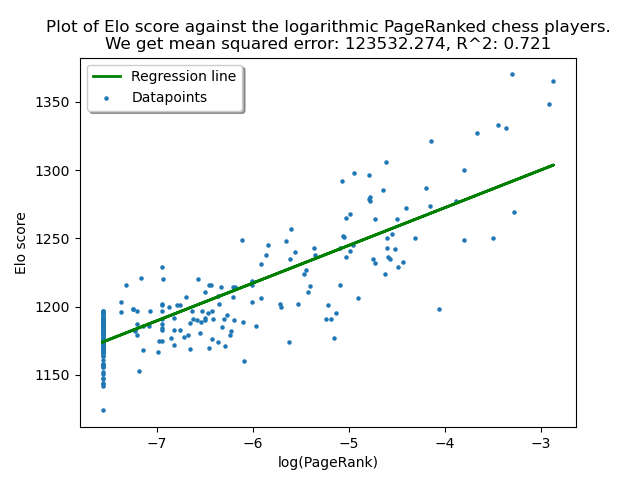
\includegraphics[width=8cm, height=7cm]{logarithmic}
        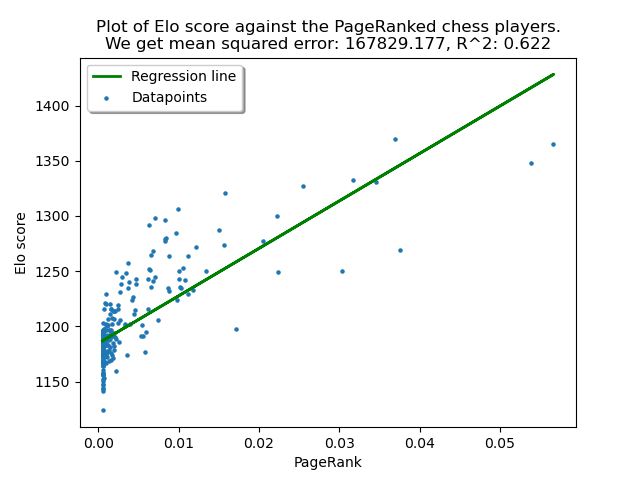
\includegraphics[width=8cm, height=7cm]{nonlogarithmic}
      \end{figure}
      What we see here is that with the logarithmic model we get a higher $R^2$ value, and a lower mean squared error which both are better in the logarithmic case than in the non logarithmic case. Taking the $R^2$ value into consideration we could say the logarithmic model is about a $10$ percent better fit.
  \newpage
  \section*{Problem2}
    \subsection*{(2a)}
      We are to show that the Maximum Likelihood estimators for the unknown parameters.
      \begin{align*}
        p(x|C_0) & = \dfrac{1}{\beta^\alpha\Gamma(\alpha)}x_{0}^{\alpha-1}e^{-x_{0}/\beta}\\
        l(\beta) & = \prod_{t=1}^{n_0} \dfrac{1}{\beta^\alpha \Gamma(\alpha)}x_{0}^{\alpha-1}e^{-x_{0}/\beta}\\
        L(\beta) & = ln(l(\beta)) = ln(\sum_{t=1}^{n_0}\dfrac{1}{\beta^\alpha \Gamma(\alpha)}x_{0}^{\alpha-1}e^{-x_{0}/\beta})\\
        & =\sum_{t=1}^{n_0}ln \left( \dfrac{1}{\beta^\alpha \Gamma(\alpha)} \right) + \sum_{t=1}^{n0}ln(x_{0}^{\alpha-1}) + \sum_{t=1}^{n_0} \dfrac{-x_0}{\beta}\\
        & = n_0( \cancelto{0}{ln(1)} - ln(\beta^\alpha) + ln(\Gamma(\alpha))) + \sum_{t=1}^{n_0} ln(x_{0}^{\alpha-1}) - \dfrac{1}{\beta}\sum_{t=1}^{n_0}x_0 \\
        \dfrac{\partial L(\beta)}{\partial\beta} & = -\dfrac{n_0 \alpha}{\beta} + \dfrac{1}{\beta^2}\sum_{t=1}^{n_0}x_0 = 0 \Leftrightarrow \dfrac{n_0 \alpha}{\beta} = \dfrac{\sum_{t=1}^{n_0}x_0}{\beta^2}\\
        \Leftrightarrow \dfrac{\beta^2}{\beta} & = \dfrac{1}{n_0 \alpha}\sum_{t=1}^{n_0}x_0 \Rightarrow \underline{\hat{\beta} = \dfrac{1}{n_0 \alpha}\sum_{t=1}^{n_0}x_0^t} \quad QED
      \end{align*}
      \begin{align*}
        p(x|C_1) & = \dfrac{1}{\sqrt{2\pi}\sigma}e^{-\dfrac{(x-\mu)^2}{2\sigma^2}} \\
        L(\mu) & = ln \left( \sum_{t=1}^{n_1} \dfrac{1}{\sqrt{2\pi}\sigma}e^{-\dfrac{(x-\mu)^2}{2\sigma^2}}\right) \\
        & = ln \left(\sum_{t=1}^{n_1} \dfrac{1}{\sqrt{2\pi}\sigma} \right) + ln\left(e^{-\dfrac{(x-\mu)^2}{2\sigma^2}} \right)\\
        & = n_1(\cancelto{0}{ln(1)}-ln(\sqrt{2\pi}) + ln(\sigma)) + \sum_{t=1}^{n_1}\dfrac{(x-\mu)^2}{2\sigma^2} \\
        & = -\dfrac{1}{2}n_1 ln(2\pi) + n_1 ln(\sigma) + \sum_{t=1}^{n_1} \dfrac{(x-\mu)^2}{2\sigma^2}
      \end{align*}
      \begin{align*}
        \dfrac{\partial L(\mu)}{\partial \mu} & =\sum_{t=1}^{n1}\dfrac{2(x - \mu)2\sigma^2 - 0}{4\sigma^2} = 0 \quad&\quad\quad \dfrac{\partial L(\sigma)}{\partial\sigma} & = \dfrac{n_1}{\sigma} + \sum_{t=1}^{n_1} \dfrac{0 - (x - \mu)^2 4\sigma}{4\sigma^4}  = 0
        \\
        & \Rightarrow \sum_{t=1}^{n_1} 2(x - \mu)2\sigma^2 = 0 \quad&\quad\quad
        \dfrac{n_1}{\sigma} & = \sum_{t=1}^{n_1} \dfrac{(x-\mu)^2}{\sigma^3}
        \\
        n_1\mu & = \sum_{t=1}^{n_1} x \quad&\quad\quad \sigma^2 &= \dfrac{1}{n_1}\sum_{t=1}^{n_1} (x-\mu)^2
        \\
        \hat{\mu} & = \dfrac{1}{n_1}\sum_{t=1}^{n_1} x_t \quad QED &\quad\quad
        \hat{\sigma}^2 &= \dfrac{1}{n_1}\sum_{t=1}^{n_1} (x_t-\mu)^2 \quad QED
      \end{align*}
    \subsection*{(2b)}
      \begin{figure}[h]
        \caption{Plot of histograms and their corresponding estimated distributions}
        \centering
        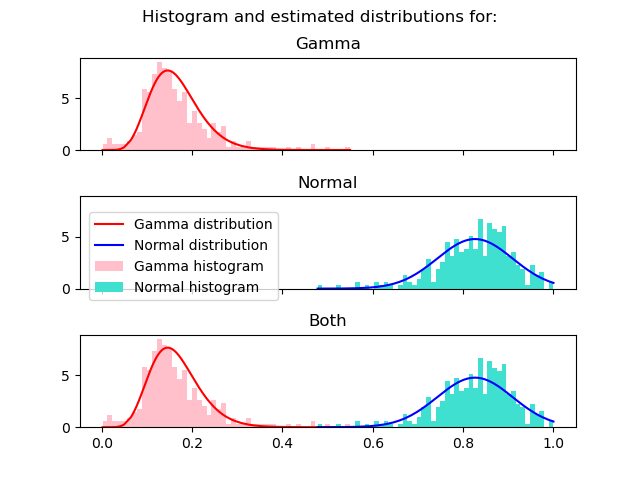
\includegraphics[width=14cm, height=10cm]{histograms}
      \end{figure}
      We see from our graph that the distributional assumptions appear to fit to our data in a reasonable manner with the estimators. The individual classified data seem not to stray too long from the distributions, but rather follow them suit.
    \subsection*{(2c)}
      Since we are only using an Bayes classifier with one attribute to classify from, some misclassfications are to be expected, actually some misclassfications are always to be expected. If we think of what the classifier does, it is basically only putting one element into one class if it is above a certain threshold value.\\
      In other words say we have a bit of a struggle with how to record or get the data in the first place. We do not know how a zero and a one is recorded, but could perhaps assume it represents a picture of either a zero or one, which then reports back the percentage of black in the picture, which again is the decimal number we are given and to work with.\\
      We can also clearly see from Figure 3 in the last plot, that some red values lie in the normal distributions classified zero's area. And the other way around.\\
      \newline
      I got the confusion matrix:
      \begin{bmatrix}
        &310 &2  \\
        &1   &300\\
      \end{bmatrix}
      , which represents:
      \begin{bmatrix}
        &tp &fn \\
        &fp &tn \\
      \end{bmatrix}\\
      \newline
      I also got accuracy $= 0.9951060358890701$, precision $= 0.9967845659163987$ and \\recall $= 0.9935897435897436$.
    \subsection*{(2d)}
      It seems i have been \textit{rickrolled}. The answer is \underline{\underline{$nevergonnagiveymuup$}}.
\end{document}
